\newpage
\section{Ôn tập chương 5}
\def\thoigian{90}%--Thời gian
\de{Đề số 1}{Chương V. Vectơ}

\begin{center}
	\textbf{PHẦN 1 - CÂU TRẮC NGHIỆM BỐN PHƯƠNG ÁN}
\end{center}
\Opensolutionfile{ans}[ans/ans-TN-ONTAPCHUONGV-DE1]
%%==========Câu 1
\begin{ex}%[0H5N1-2]%[Dự án D - đợt 2 NH24-25- Quang Vinh NT]
	Phát biểu nào sau đây là \textbf{sai}?
	\choice
	{Hai vectơ cùng phương là hai vectơ có giá song song hoặc trùng nhau}
	{Nếu hai vectơ cùng hướng thì chúng có cùng phương}
	{Vectơ-không cùng phương với mọi vectơ}
	{\True Nếu hai vectơ cùng phương thì chúng cùng hướng}
	\loigiai
	{Hai vectơ cùng phương thì chúng có thể cùng hướng hoặc ngược hướng.}
\end{ex}

%%==========Câu 2
\begin{ex}%[0H5H1-3]%[Dự án D - đợt 2 NH24-25- Quang Vinh NT]
	Cho $M$ là trung điểm của đoạn thẳng $AB$. Khẳng định nào sau đây là đúng?
	\choice
	{$\overrightarrow{AB}$ và $\overrightarrow{MB}$ ngược hướng}
	{$\left|\overrightarrow{AB}\right|=\left|\overrightarrow{MB}\right|$}
	{$\overrightarrow{MA}=\overrightarrow{MB}$}
	{\True $\overrightarrow{AB}$ và $\overrightarrow{AM}$ cùng phương}
	\loigiai{
		\begin{center}
			\begin{tikzpicture}[font=\footnotesize, line join=round, line cap=round, >=stealth]
				\path 	(0,0) coordinate (A)
				(4,0) coordinate (B)
				(2,0) coordinate (M);
				\draw 	(A)--(B);
				\foreach \x /\goc in {A/180,B/0,M/-90}
				\fill[black] (\x) circle (1pt)
				($(\x)+(\goc:3mm)$) node {$\x$};
			\end{tikzpicture}		
		\end{center}
		Khi $M$ là trung điểm của đoạn thẳng $AB$ thì $\overrightarrow{AB}$ và $\overrightarrow{AM}$ cùng phương.
	}
\end{ex}
%%==========Câu 3
\begin{ex}%[0H5H1-5]%[Dự án D - đợt 2 NH24-25- Quang Vinh NT]
	Cho hình chữ nhật $ABCD$ có $AB=a$, $AD=2a$. Tính $\left|\overrightarrow{AC}\right|$.
	\choice
	{$3a$}
	{\True $\sqrt{5}a$}
	{$\sqrt{2}a$}
	{$2a$}
	\loigiai{
		\begin{center}
			\begin{tikzpicture}[scale=0.8, font=\footnotesize,line join=round, line cap=round, >=stealth,rotate=90]
				\def\a{2} %%chiều dài
				\def\b{4} %%chiều rộng
				\path 
				(0,0) coordinate (A)
				(\a,0) coordinate (B)
				(0,-\b) coordinate (D)
				($(B)+(D)-(A)$) coordinate (C)
				($(B)!1/2!(C)$) coordinate (M)
				($(C)!1/3!(D)$) coordinate (N)
				;
				\draw (A)--(C);
				\draw (A)--(B) node[midway,left]{$a$}
				(A)--(D) node[midway,below]{$2a$}
				(D)--(C)--(B)
				;
				\foreach \x/\y/\z in {A/B/C, D/A/B, D/C/B, C/D/A}
				{pic[draw,angle eccentricity=1.8,angle radius=2mm]{right angle = \x--\y--\z}}
				;
				\foreach \i/\g in {A/90,B/90,C/-90,D/-90}
				\fill[black] (\i) circle(1pt)+(\g:3mm)node[scale=1]{$\i$};
			\end{tikzpicture}
		\end{center}
		Ta có $\left|\overrightarrow{AC}\right|=AC$.\\
		Xét tam giác vuông $ABC$ ta có $AC=\sqrt{AB^2+BC^2}=\sqrt{a^2+(2a)^2}=\sqrt{5}a$.
	}
\end{ex}
%%==========Câu 4
\begin{ex}%[0H5H2-1]%[Dự án D - đợt 2 NH24-25- Quang Vinh NT]
	Trong mặt phẳng, cho năm điểm phân biệt $A$, $B$, $C$, $D$, $E$. Vectơ $\overrightarrow{u}=\overrightarrow{BD}+\overrightarrow{EA}+\overrightarrow{CE}-\overrightarrow{CD}$ bằng vectơ nào sau đây?
	\choice
	{$\overrightarrow{BD}$}
	{\True $\overrightarrow{BA}$}
	{$\overrightarrow{AE}$}
	{$\overrightarrow{AB}$}
	\loigiai{
		Ta có
		\begin{align*}
			\overrightarrow{u}&= \overrightarrow{BD}+\overrightarrow{EA}+\overrightarrow{CE}-\overrightarrow{CD}\\
			&=\overrightarrow{BD}+\overrightarrow{EA}+\left(\overrightarrow{CE}-\overrightarrow{CD}\right)\\
			&=\overrightarrow{BD}+\overrightarrow{EA}+\overrightarrow{DE} \\
			&=\left(\overrightarrow{BD}+\overrightarrow{DE}\right)+\overrightarrow{EA}\\
			&= \overrightarrow{BE}+\overrightarrow{EA}=\overrightarrow{BA}.
		\end{align*} 
	}
\end{ex}
%%==========Câu 5
\begin{ex}%[0H5H2-1]%[Dự án D - đợt 2 NH24-25- Quang Vinh NT]
	\immini{Cho hình lục giác đều $ABCDEF$ tâm $O$. Khẳng định nào dưới đây đúng?
		\choice
		{\True $\overrightarrow{AB}+\overrightarrow{AF}=\overrightarrow{AO}$}
		{$\overrightarrow{AB}+\overrightarrow{AF}=\overrightarrow{DO}$}
		{$\overrightarrow{AB}+\overrightarrow{AF}=\overrightarrow{CO}$}
		{$\overrightarrow{AB}+\overrightarrow{AF}=\overrightarrow{OA}$}}{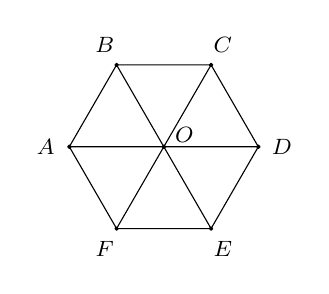
\begin{tikzpicture}[scale=0.6, font=\footnotesize, line join=round, line cap=round, >=stealth]
			\coordinate (O) at (0,0);
			\foreach \x/\y in {A/180,B/120,C/60,D/0,E/-60,F/-120} {
				\coordinate (\x) at (\y:2);
				\draw[fill=black] (\x) circle(1pt) node [shift={(\y:.3)}] {$\x$};}
			\draw[fill=black] (O) circle(1pt) node[shift={(30:.3)}] {$O$};
			\draw (A)--(B)--(C)--(D)--(E)--(F)--cycle;
			\draw (A)--(D) (B)--(E) (C)--(F);
	\end{tikzpicture}}
	\loigiai{Ta có $\overrightarrow{AB}+\overrightarrow{AF}=\overrightarrow{AB}+\overrightarrow{BO}=\overrightarrow{AO}$.
	}
\end{ex}
%%==========Câu 6
\begin{ex}%[0H5H2-4]%[Dự án D - đợt 2 NH24-25- Quang Vinh NT]
	Cho hình vuông $ABCD$ có độ dài cạnh bằng $5$. Hãy tính $\left|\overrightarrow{AB}+\overrightarrow{AD}\right|$.
	\choice
	{$10\sqrt 2 $}
	{$10$}
	{$5$}
	{\True $5\sqrt 2 $}
	\loigiai{
		Ta có $\left|\overrightarrow{AB}+\overrightarrow{AD}\right|=\left|\overrightarrow{AC}\right|=AC=5\sqrt{2}$.
	}
\end{ex}
%%==========Câu 7
\begin{ex}%[0H5H3-2]%[Dự án D - đợt 2 NH24-25- Quang Vinh NT]
	Cho hình chữ nhật $ABCD$ có $E$ là trung điểm $BC$. Khi đó $\overrightarrow{u} = \overrightarrow{BA} + 2\overrightarrow{EC}$	bằng vectơ nào sau đây?
	\choice
	{$\overrightarrow{DB} $}
	{\True $\overrightarrow{BD} $}
	{$\overrightarrow{DE} $}
	{$\overrightarrow{AC} $}
	\loigiai{
		\immini{Ta có $\overrightarrow{u} = \overrightarrow{BA} + 2\overrightarrow{EC}=\overrightarrow{BA} + \overrightarrow{BC}=\overrightarrow{BD}$.}{\begin{tikzpicture}[rotate=0,scale=0.4, font=\footnotesize,line join=round, line cap=round, >=stealth]
				\path 
				(0,0) coordinate (A)
				++(90:6) coordinate (B)
				++(0:8) coordinate (C)
				($(A)+(C)-(B)$) coordinate (D)
				($(B)!1/2!(C)$) coordinate (E)
				;
				%\foreach \i in {A,B,C,D}{
					%	\coordinate (\i') at ($(\i)+(1,4)$);
					%}
				%\draw (A')--(B')--(C')--(D')--cycle;
				\draw (A)--(B)--(C)--(D)--cycle  (B)--(D);			
				\foreach \i/\g/\t in {A/180/A,B/180/B,C/0/C,D/0/D,E/90/E}
				\fill[black] (\i) circle(1.5pt)+(\g:5mm)node[scale=1]{$\t$};
		\end{tikzpicture}}
	}
\end{ex}
%%==========Câu 8
\begin{ex}%[0H5H3-1]%[Dự án D - đợt 2 NH24-25- Quang Vinh NT]
	Cho tam giác $ABC$ đều cạnh bằng $1$, trọng tâm $G$. Độ dài vectơ $\overrightarrow{AG}$ bằng
	\choice
	{$\dfrac{\sqrt{3}}{2}$}
	{\True $\dfrac{\sqrt{3}}{3}$}
	{$\dfrac{\sqrt{3}}{4}$}
	{$\dfrac{\sqrt{3}}{6}$}
	\loigiai{
		Gọi $M$ là trung điểm của $BC$, ta có $\left|\overrightarrow{AG}\right|=AG=\dfrac{2}{3}AM=\dfrac{2}{3}\cdot\dfrac{\sqrt{3}}{2}=\dfrac{\sqrt{3}}{3}$.
	}
\end{ex}
%%==========Câu 9
\begin{ex}%[0H5V3-9]%[Dự án D - đợt 2 NH24-25- Quang Vinh NT]
	Cho ba lực $\overrightarrow{F}_1=\overrightarrow{MA}$, $\overrightarrow{F}_2=\overrightarrow{MB}$, $\overrightarrow{F}_3=\overrightarrow{MC}$ cùng tác động vào một vật tại điểm $M$ và vật đứng yên. 
	\immini{Cho biết cường độ của $\overrightarrow{F}_1$, $\overrightarrow{F}_2$ đều bằng $ 100$ N và $\widehat{AMB}=60^\circ $. Khi đó cường độ lực của $\overrightarrow{F}_3$ bằng
		\choice
		{$50\sqrt{2}$ N}
		{$50\sqrt{3}$ N}
		{$25\sqrt{3}$ N}
		{\True $ 100\sqrt{3}$ N} }{
		\begin{tikzpicture}[scale=0.6, font=\footnotesize, line join=round, line cap=round, >=stealth]
			\path
			(0:0) coordinate (M)
			(30:2) coordinate (A)
			(-30:2) coordinate (B)
			(180:3) coordinate (C)
			($(M)!0.5!(A)$) coordinate (d)
			($(M)!0.5!(B)$) coordinate (e)
			($(M)!0.5!(C)$) coordinate (f)
			;
			\draw[->] (M)--(A);
			\draw[->] (M)--(B);
			\draw[->] (M)--(C);	
			\fill[black] (M) circle(1pt) node[above left]{$M$};
			\draw
			(A) node[above right]{$A$}
			(B) node[below right]{$B$}
			(C) node[left]{$C$}
			(d) node[above left]{$\overrightarrow{F}_1$}
			(e) node[below left]{$\overrightarrow{F}_2$}
			(f) node[above]{$\overrightarrow{F}_3$}
			;	
		\end{tikzpicture}
	}
	\loigiai{\immini{
			Gọi $O$ là trung điểm của đoạn thẳng $AB$.\\ Khi đó hợp lực  $\overrightarrow{F}_1+\overrightarrow{F}_2=\overrightarrow{MA}+\overrightarrow{MB}=2\overrightarrow{MO}$.\\
			Ta có $MO=\dfrac{100\sqrt{3}}{2}=50\sqrt{3}$.\\
			Vậy hợp lực $\overrightarrow{F}_1+\overrightarrow{F}_2=2\dot 50\sqrt{3}= 100\sqrt{3}$ N.\\
			Vì điểm $M$ đứng yên nên độ lớn của lực $\overrightarrow{F}_3$ là $100\sqrt{3}$ N.
		}	
		{\begin{tikzpicture}[scale=0.8, font=\footnotesize, line join=round, line cap=round, >=stealth]
				\path
				(0:0) coordinate (M)
				(30:3) coordinate (A)
				(-30:3) coordinate (B)
				(180:3) coordinate (C)
				($(M)!0.5!(A)$) coordinate (d)
				($(M)!0.5!(B)$) coordinate (e)
				($(M)!0.5!(C)$) coordinate (f)
				($(A)!0.5!(B)$) coordinate (O);
				\draw[->] (M)--(A);
				\draw[->] (M)--(B);
				\draw[->] (M)--(C);
				\draw (A)--(B);
				\fill[black] (M) circle(1pt) node[above]{$M$};
				\fill[black] (O) circle(1pt) node[below left]{$O$};
				\fill[black] (A) circle(1pt) node[above]{$A$};
				\fill[black] (B) circle(1pt) node[below]{$B$};
				\draw
				(C) node[left]{$C$}
				(d) node[above left]{$\overrightarrow{F}_1$}
				(e) node[below left]{$\overrightarrow{F}_2$}
				(f) node[above]{$\overrightarrow{F_3}$}
				;					
				\draw (M)--(O);
				\draw[-] ($(M)!4mm!(B)$) to[bend right=45] node[pos=.1,right]{$60^\circ$} ($(M)!4mm!(A)$);
	\end{tikzpicture}}}
	
\end{ex}
%%==========Câu 10
\begin{ex}%[0H5H4-1]%[Dự án D - đợt 2 NH24-25- Quang Vinh NT]
	Cho $\overrightarrow{a}$ và $\overrightarrow{b}$ là hai vectơ cùng hướng và đều khác vectơ $\overrightarrow{0}$. Mệnh đề nào sau đây đúng?
	\choice
	{\True $\overrightarrow{a}\cdot\overrightarrow{b}=\left|\overrightarrow{a}\right|\cdot\left|\overrightarrow{b}\right|$}
	{$\overrightarrow{a}\cdot\overrightarrow{b}=0$}
	{$\overrightarrow{a}\cdot\overrightarrow{b}=-1$}
	{$\overrightarrow{a}\cdot\overrightarrow{b}=-\left|\overrightarrow{a}\right|\cdot\left|\overrightarrow{b}\right|$}
	\loigiai{
		Vì $\overrightarrow{a}$ và $\overrightarrow{b}$ cùng hướng nên $\left(\overrightarrow{a},\overrightarrow{b}\right)=0^\circ$. Do đó $\overrightarrow{a}\cdot\overrightarrow{b}=\left|\overrightarrow{a}\right|\cdot\left|\overrightarrow{b}\right|\cdot \cos 0^\circ=\left|\overrightarrow{a}\right|\cdot\left|\overrightarrow{b}\right|$.
	}
\end{ex}
%%==========Câu 11
\begin{ex}%[0H5H4-1]%[Dự án D - đợt 2 NH24-25- Quang Vinh NT]
	Cho hình vuông $ABCD$ cạnh $a$. Tính tích vô hướng $\overrightarrow{AB} \cdot \overrightarrow{AD}$.
	\choice
	{$\overrightarrow{AB} \cdot \overrightarrow{AD}=-a$}
	{$\overrightarrow{AB} \cdot \overrightarrow{AD}=2a^2$}
	{$\overrightarrow{AB} \cdot \overrightarrow{AD}=\dfrac{1}{2}a^2$}
	{\True $\overrightarrow{AB} \cdot \overrightarrow{AD}=0$}
	\loigiai{
		Vì $AB \perp AD$ nên $\overrightarrow{AB} \cdot \overrightarrow{AD}=0$.
	}
\end{ex}
%%==========Câu 12
\begin{ex}%[0H5H4-2]%[Dự án D - đợt 2 NH24-25- Quang Vinh NT]
	Cho hai vectơ $\overrightarrow{a}$ và $\overrightarrow{b}$ thỏa mãn $\left|\overrightarrow{a}\right|=3$, $\left|\overrightarrow{b}\right|=2$ và $\overrightarrow{a}\cdot\overrightarrow{b}=-3$. Khi đó góc $\alpha$ giữa hai vectơ $\overrightarrow{a}$ và $\overrightarrow{b}$ bằng 
	\choice
	{$30^\circ$}
	{$45^\circ$}
	{$60^\circ$}
	{\True $120^\circ$}
	\loigiai{
		Ta có $\overrightarrow{a}\cdot\overrightarrow{b}=\left|\overrightarrow{a}\right|\cdot\left|\overrightarrow{b}\right|\cdot \cos\alpha\Leftrightarrow -3=3\cdot 2\cdot\cos\alpha\Leftrightarrow\cos\alpha=-\dfrac{1}{2}\Rightarrow\alpha=120^\circ$.
	}
\end{ex}
\Closesolutionfile{ans}
%\begin{center}
%	\textbf{ĐÁP ÁN}
%	\inputansbox{10}{ans/ans}	
%\end{center}

\begin{center}
	\textbf{PHẦN 2 - CÂU TRẮC NGHIỆM ĐÚNG SAI}
\end{center}

\Opensolutionfile{ans}[ans/answer-DS-ONTAPCHUONGV-DE1]
%%==========Câu 13
\begin{ex}%[0H5V2-6]%[Dự án D - đợt 2 NH24-25- Quang Vinh NT]
	Cho điểm $A$ khi tác động vật lý bằng $3$ lực $\overrightarrow{F}_1$, $\overrightarrow{F}_2$, $\overrightarrow{F}_3$ như hình bên dưới thì vật đó đứng yên. Coi ma sát không đáng kể và lực ngoại cảnh không ảnh hưởng gì đến chất điểm $A$. Biết $\overrightarrow{F}_{3}$ có độ lớn bằng $30$ N, tính độ lớn các lực $\overrightarrow{F}_{1}$, $\overrightarrow{F}_{2}$.
	\begin{center}
		\begin{tikzpicture}[font=\footnotesize, line join=round, line cap=round, >=stealth, scale=1]
			\path[draw] (0,0)coordinate(A) (4,0)coordinate(Q) (0,-2)coordinate(M) (4,-2)coordinate(R) ($(A)!-1!(R)$)coordinate(K)
			(0,-1)coordinate(F1) (-1,0.7)coordinate(F2) (2,0)coordinate(F3);
			\draw[->] (A)--(Q);
			\draw[->] (A)--(R);
			\draw[->] (A)--(M);
			\draw[->] (A)--(K);
			\draw (Q)--(R)--(M);
			\draw (F1) node[left,black]{$\overrightarrow{F}_{1}$};
			\draw (F2) node[left,black,above]{$\overrightarrow{F}_{2}$};
			\draw (F3) node[left,black,above]{$\overrightarrow{F}_{3}$};
			\foreach \a/\b/\c in {M/A/Q} {
				\draw pic[draw, angle radius=0.2cm]{right angle=\a--\b--\c};
			}
			\foreach \d/\g in {A/-120,Q/0,R/0,M/-90} 
			\fill[black](\d) circle (1.5pt)+(\g:.3)node{$\d$};
			\draw pic[draw, angle radius=0.2cm]{ angle=F2--A--M};
			\node at ($(A)+(180:7mm)$) {$120^{\circ}$};
		\end{tikzpicture}
	\end{center}
	\choiceTF
	{\True  $\left|\overrightarrow{F}_{1}\right|=10\sqrt{3}$}
	{$\overrightarrow{F}_{1}+ \overrightarrow{F}_{2}=\overrightarrow{F}_{3}$}
	{$\left|\overrightarrow{F}_{2}\right|=10\sqrt{3}$}
	{$\left|\overrightarrow{F}_{1}\right|=\left|\overrightarrow{F}_{2}\right|$}
	\loigiai{
		\begin{center}
			\begin{tikzpicture}[font=\footnotesize, line join=round, line cap=round, >=stealth, scale=1]
				\path[draw] (0,0)coordinate(A) (4,0)coordinate(Q) (0,-2)coordinate(M) (4,-2)coordinate(R) ($(A)!-1!(R)$)coordinate(K)
				(0,-1)coordinate(F1) (-1,0.7)coordinate(F2) (2,0)coordinate(F3);
				\draw[->] (A)--(Q);
				\draw[->] (A)--(R) node[midway,above,sloped,black]{$\overrightarrow{F}_{4}$};
				\draw[->] (A)--(M);
				\draw[->] (A)--(K);
				\draw (Q)--(R)--(M);
				\draw (F1) node[left,black]{$\overrightarrow{F}_{1}$};
				\draw (F2) node[left,black,above]{$\overrightarrow{F}_{2}$};
				\draw (F3) node[left,black,above]{$\overrightarrow{F}_{3}$};
				\foreach \a/\b/\c in {M/A/Q} {
					\draw pic[draw, angle radius=0.2cm]{right angle=\a--\b--\c};
				}
				\foreach \d/\g in {A/-120,Q/0,R/0,M/-90} 
				\fill[black](\d) circle (1.5pt)+(\g:.3)node{$\d$};
				\draw pic[draw, angle radius=0.2cm]{ angle=F2--A--M};
				\node at ($(A)+(180:7mm)$) {$120^{\circ}$};
			\end{tikzpicture}
		\end{center}
		Ta gọi $\overrightarrow{F}_{1}+ \overrightarrow{F}_{3}=\overrightarrow{F}_{4}$.
		
		Mà $\overrightarrow{F}_{1}+ \overrightarrow{F}_{2}+\overrightarrow{F}_{3}=\overrightarrow{0} \Leftrightarrow \overrightarrow{F}_{4}=-\overrightarrow{F}_{2} \Rightarrow \left|\overrightarrow{F}_{4}\right| = \left|\overrightarrow{F}_{2}\right|$.
		
		\begin{itemchoice}
			\itemch Ta có $\left|\overrightarrow{F}_{1}\right| = \left|\overrightarrow{F}_{3}\right| \cdot \tan 30^{\circ} = 30 \cdot \dfrac{1}{\sqrt{3}} = 10\sqrt{3}$ N.
			\itemch Do vật đứng yên nên $\overrightarrow{F}_{1}+ \overrightarrow{F}_{2}+ \overrightarrow{F}_{3} = \overrightarrow{0}$ hay $\overrightarrow{F}_{1}+ \overrightarrow{F}_{2} = -\overrightarrow{F}_{3}$.
			\itemch Ta có $\left|\overrightarrow{F}_{2}\right| = \left|\overrightarrow{F}_{4}\right| = \sqrt{\left|\overrightarrow{F}_{1}\right|^{2} + \left|\overrightarrow{F}_{3}\right|^{2}} = \sqrt{(10\sqrt{3})^2 + 30^2} = 20\sqrt{3}$ N.
			\itemch Ta thấy $\left|\overrightarrow{F}_{1}\right| \neq \left|\overrightarrow{F}_{2}\right|$.
		\end{itemchoice}
	}
\end{ex}


%%==========Câu 14
	\begin{ex}%[0H5H3-5]%[Dự án D - đợt 2 NH24-25- Quang Vinh NT]
	Cho hình bình hành $ABCD$ có tâm $O$, $G$ là trọng tâm tam giác $ABC$ và $N$ là trung điểm $AB$.
	\choiceTF
	{$\overrightarrow{BO} + \overrightarrow{OD} = \overrightarrow{0}$}
	{\True $\overrightarrow{AB} + \overrightarrow{AD} = \overrightarrow{AC}$}
	{$\overrightarrow{BG} = \dfrac{2}{3}\left(\overrightarrow{BA} + \overrightarrow{BC} \right)$}
	{\True Nếu $\overrightarrow{AB} = x\overrightarrow{BO} + y\overrightarrow{CN}$ thì $x + y = -2$}
	\loigiai{
		\begin{itemchoice}
			\immini{
				\itemch Ta có $\overrightarrow{BO} + \overrightarrow{OD} = \overrightarrow{BD}$.\\
				Mà $B$, $D$ là hai điểm phân biệt trên hình bình hành $ABCD$ nên $\overrightarrow{BD} \neq \overrightarrow{0}$.\\
				Do đó $\overrightarrow{BO} + \overrightarrow{OD} \neq \overrightarrow{0}$.
				\itemch Xét hình bình hành $ABCD$, áp dụng quy tắc hình bình hành, ta có $$\overrightarrow{AB} + \overrightarrow{AD} = \overrightarrow{AC}.$$
			}{
				\begin{tikzpicture}[>=stealth,line join=round,line cap=round,font=\footnotesize,scale=1]
					\path 
					(0,0) coordinate (A)
					(-1,-2) coordinate (B)
					(2.5,-2) coordinate (C)
					($(A)-(B)+(C)$) coordinate (D)
					($(A)!0.5!(B)$) coordinate (N)
					($(A)!0.5!(C)$) coordinate (O)
					($(B)!2/3!(O)$) coordinate (G)
					;
					\draw 
					(A)--(B)--(C)--(D)--(A)--(C)--(N) (B)--(D);
					\foreach \p/\g in {B/-90, D/90, A/90, C/-90,N/180,G/-90,O/80}
					\draw[fill=black] (\p) circle (1pt) node[shift=(\g:3mm)] {$\p$};
				\end{tikzpicture}
			}
			\itemch Vì $O$ là tâm của hình bình hành $ABCD$ nên $O$ là trung điểm của $AC$.\\
			Khi đó, ta có $\overrightarrow{BA} + \overrightarrow{BC} = 2\overrightarrow{BO} + \left(\overrightarrow{OA} + \overrightarrow{OC}\right) = 2\overrightarrow{BO} + \overrightarrow{0} = 2\overrightarrow{BO}$.\\
			Suy ra $\overrightarrow{BO} = \dfrac{1}{2}\left(\overrightarrow{BA} + \overrightarrow{BC}\right)$.\\
			Vì $G$ là trọng tâm $\triangle ABC$ nên $\overrightarrow{BG} = \dfrac{2}{3}\overrightarrow{BO} = \dfrac{2}{3}\cdot \dfrac{1}{2}\left(\overrightarrow{BA} + \overrightarrow{BC}\right) = \dfrac{1}{3}\left(\overrightarrow{BA} + \overrightarrow{BC}\right)$.
			\itemch Ta có
			\allowdisplaybreaks
			\begin{eqnarray*}
				\overrightarrow{BO} + \overrightarrow{CN} &=& \overrightarrow{BA} + \overrightarrow{AO} + \overrightarrow{CA} + \overrightarrow{AN}\\
				&=& -\overrightarrow{AB} + \dfrac{1}{2}\overrightarrow{CA} + \dfrac{1}{2}\overrightarrow{AB}\\
				&=& -\dfrac{1}{2}\overrightarrow{AB} + \dfrac{1}{2}\left(\overrightarrow{CN} + \overrightarrow{NA}\right)\\
				&=& -\dfrac{1}{2}\overrightarrow{AB} + \dfrac{1}{2}\left(\overrightarrow{CN} + \dfrac{1}{2}\overrightarrow{BA}\right)\\
				&=& -\dfrac{3}{4}\overrightarrow{AB} + \dfrac{1}{2}\overrightarrow{CN}\\
				\Rightarrow \dfrac{3}{4}\overrightarrow{AB} &=& -\overrightarrow{BO} - \dfrac{1}{2}\overrightarrow{CN}\\
				\Rightarrow \overrightarrow{AB} &=& -\dfrac{4}{3}\overrightarrow{BO} - \dfrac{2}{3}\overrightarrow{CN}.
			\end{eqnarray*}
			Do đó $x = -\dfrac{4}{3}$ và $y = -\dfrac{2}{3}$ suy ra $x + y = -\dfrac{4}{3} + \left( -\dfrac{2}{3}\right) = -2$.
		\end{itemchoice}
	}
\end{ex}
\Closesolutionfile{ans}
%\inputansbox[2]{2}{ans/answer.tex}

\begin{center}
	\textbf{PHẦN 3 - CÂU TRẮC NGHIỆM TRẢ LỜI NGẮN}
\end{center}
\setcounter{ex}{0}
\Opensolutionfile{ans}[ans-KQ-ONTAPCHUONGV-DE1]

%%==========Câu 1
\begin{ex}%[0H5V2-6]%[Dự án D - đợt 2 NH24-25- Quang Vinh NT]
	Trên mặt phẳng, chất điểm $A$ chịu tác dụng của ba lực $\overrightarrow{F}_1$, $\overrightarrow{F}_2$, $\overrightarrow{F}_3$ và ở trạng thái cân bằng. Góc giữa hai vectơ $\overrightarrow{F}_1$, $\overrightarrow{F}_2$ bằng $120^{\circ}$. Tính độ lớn của $\overrightarrow{F}_3$ (làm tròn đến hàng phần trăm), biết $\left| \overrightarrow{F}_1\right| =\left| \overrightarrow{F}_2\right| =2 \sqrt{5}$ N.
	
	\shortans[oly]{$4{,}47$}
	\loigiai{
		\immini{Vì chất điểm $A$ chịu tác dụng của ba lực $\overrightarrow{F}_1$, $\overrightarrow{F}_2$, $\overrightarrow{F}_3$ và ở trạng thái cân bằng nên ta có 
			\begin{eqnarray*}
				&&\overrightarrow{F}_1+\overrightarrow{F}_2+\overrightarrow{F}_3=\overrightarrow{0}\\
				&\Rightarrow& \overrightarrow{F}+\overrightarrow{F}_{3}=\overrightarrow{0}\\
				&\Rightarrow& \left| \overrightarrow{F}\right| =\left| \overrightarrow{F}_{3}\right|\\
				&\Rightarrow& F=F_{3}.  
			\end{eqnarray*} 
			Áp dụng định lý côsin vào $\triangle MAD$ ta có
			\begin{eqnarray*}
				&&AD^{2}=MA^{2}+MD^{2}-2MA\cdot MD\cdot \cos \widehat{AMD}\\
				&\Rightarrow& F_{2}^{2}=F_{1}^{2}+F^{2}-2\cdot F_{1}\cdot F\cdot\cos60^{\circ}\\
				&\Rightarrow&F^{2}-2\cdot F_{1}\cdot F\cdot\cos60^{\circ}=0\\
				&\Rightarrow&F^{2}-2\sqrt{5}\cdot F=0\\
				&\Rightarrow& \hoac{&F=0 &\text{(loại)}\\&F=2\sqrt{5}&\text{(nhận)}.}
			\end{eqnarray*}
			Vậy $F=2\sqrt{5}\approx 4{,}47$ N.}{
			\begin{tikzpicture}[>=stealth,line join=round,line cap=round,font=\footnotesize,scale=1]
				\path (0,0) coordinate (M)
				(-60:3) coordinate (B)
				(60:3) coordinate (A)
				($(A)+(B)-(M)$) coordinate (D)
				($(D)!2!(M)$) coordinate (C) 
				;
				\draw[->] (M)--(C)node[midway,above]{$\overrightarrow{F}_3$}; 
				\draw[->] (M)--(A)node[midway,left]{$\overrightarrow{F}_1$}; 
				\draw[->] (M)--(B)node[midway,left]{$\overrightarrow{F}_2$};
				\draw[->] (M)--(D)node[midway,above]{$\overrightarrow{F}$};  
				%\draw (M) node[right=0.3]{$120^{\circ}$};
				\draw[dashed] (A)--(D)--(B);
				\foreach \x/\g in {A/135, B/0, C/180, D/0, M/120}{\draw[fill=black] (\x) circle (1pt) node[shift={(\g:7pt)},font=\footnotesize]{$\x$};}
		\end{tikzpicture}}
	}
\end{ex}

%%==========Câu 2
\begin{ex}%[0H5V3-5]%[Dự án D - đợt 2 NH24-25- Quang Vinh NT]
	Cho tam giác $ABC$. Gọi $M$ là một điểm trên cạnh $BC$ sao cho $MB=2MC$. Phân tích $\overrightarrow{AM} = m\overrightarrow{AB} + n\overrightarrow{AC}$. Tính $P = 3m+6n$.
	
	\shortans[oly]{$5$}
	\loigiai{
		\begin{center}
				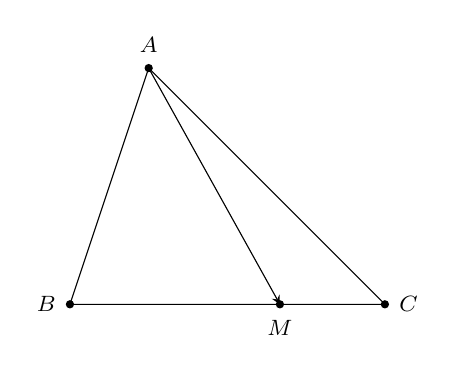
\begin{tikzpicture}[font=\footnotesize, line join=round, line cap=round, >=stealth, scale=1]
				\path (0,0) coordinate(B)
				--++(4,0) coordinate(C)
				(1,3)coordinate(A)
				(B)--(C)coordinate[pos=2/3](M);
				\draw (A)--(B)--(C)--cycle;
				\draw[->](A)--(M);		
				\foreach \d/\g in {A/90,B/180,C/0,M/-90	}\fill[black](\d) circle (1.5pt)+(\g:.3)node{$\d$};
			\end{tikzpicture}
		\end{center}
		Ta có $\overrightarrow{AM} = \overrightarrow{AB} + \overrightarrow{BM} = \overrightarrow{AB} +\dfrac{2}{3}\cdot \overrightarrow{BC}=\overrightarrow{AB} +\dfrac{2}{3}\cdot \overrightarrow{BA} +\dfrac{2}{3}\cdot \overrightarrow{AC}=\dfrac{1}{3}\cdot \overrightarrow{AB} +\dfrac{2}{3}\cdot \overrightarrow{AC}$.\\
		Vậy $P = 3m+6n= 3\cdot \dfrac{1}{3}+6\cdot \dfrac{2}{3}=5$.
	}
\end{ex}
%%==========Câu 3
\begin{ex}%[0H5H4-1]%[Dự án D - đợt 2 NH24-25- Quang Vinh NT]
	Cho hình chữ nhật $ABCD$ có $AB=8, AD=6$.  Tính $\overrightarrow{AB}\cdot\overrightarrow{BD}$.
	
	\shortans[oly]{$-64$}
	\loigiai{
		\begin{center}
			\begin{tikzpicture}[scale=1, font=\footnotesize, line join=round, line cap=round, >=stealth]
				%Hình 1
				\path (0,0) coordinate(A) 
				(3,0) coordinate(B)
				(3,-2) coordinate(C)
				(0,-2) coordinate(D)
				;
				\foreach \p/\g in {A/90, B/90, C/-90, D/-90}
				\draw[fill=black] (\p) circle(1pt) node [shift={(\g:.3)}] {$\p$};
				\draw (A)--(B)--(C)--(D)--cycle;
				\foreach \a/\b/\c in {B/A/D} {
					\draw pic[draw, angle radius=0.2cm]{right angle=\a--\b--\c};
				}
			\end{tikzpicture}
		\end{center}
		Ta có \[\overrightarrow{AB}\cdot\overrightarrow{BD} = \overrightarrow{AB}\cdot\left(\overrightarrow{AD}-\overrightarrow{AB}\right) =\overrightarrow{AB}\cdot \overrightarrow{AD}-\overrightarrow{AB}^2=-AB^2=-64.\]
	}
\end{ex}
%%==========Câu 4

\begin{ex}%[0H5H4-2]%[Dự án D - đợt 2 NH24-25- Quang Vinh NT]
	Cho hai vectơ $\overrightarrow{u}$ và $\overrightarrow{v}$ thỏa $|\overrightarrow{u}|=3$, $|\overrightarrow{v}|=4$ và $|2 \overrightarrow{u}-\overrightarrow{v}|=\sqrt{76}$. Góc giữa hai vectơ $\overrightarrow{u}$ và $\overrightarrow{v}$ bằng bao nhiêu độ?
	
	\shortans[oly]{120}
	\loigiai{
		Ta có $|2 \overrightarrow{u}-\overrightarrow{v}|=\sqrt{76}\Leftrightarrow 4\cdot \overrightarrow{u}^2-4\overrightarrow{ u}\cdot \overrightarrow{v}+\overrightarrow{v}^2=76\Leftrightarrow \overrightarrow{ u}\cdot \overrightarrow{v}=-6$.\\
		Mặt khác $\overrightarrow{ u}\cdot \overrightarrow{v}=|\overrightarrow{u}|\cdot |\overrightarrow{v}|\cdot \cos (\overrightarrow{u}, \overrightarrow{v})\Rightarrow \cos\left(\overrightarrow{u},\overrightarrow{v}\right)=\dfrac{\overrightarrow{u}\cdot \overrightarrow{v}}{|\overrightarrow{u}|\cdot |\overrightarrow{v}|}=\dfrac{-6}{3\cdot 4}=-\dfrac{1}{2}$.\\
		Suy ra $\left(\overrightarrow{u},\overrightarrow{v}\right)=120^{\circ}$.
	}
\end{ex}
\Closesolutionfile{ans}

\begin{center}
	\textbf{PHẦN 4 - TỰ LUẬN}
\end{center}
\Opensolutionfile{ans}[ans-TL-ONTAPCHUONGV-DE1]
%%==========Câu 1
\begin{ex}%[0H5H3-6]%[Dự án D - đợt 2 NH24-25- Quang Vinh NT]
	Cho hình chữ nhật $ABCD$ biết $BC=a$, $CD=5a$. Gọi $N$ là trung điểm của cạnh $AD$ và $M$ thuộc cạnh $BC$ sao cho $BC=3MB$. Tính độ dài của vectơ $\overrightarrow{a}=\overrightarrow{BN}+3\overrightarrow{MB}$.
	\loigiai{
		\immini{
			Ta có $\overrightarrow{a}=\overrightarrow{BN}+3 \overrightarrow{MB}=\overrightarrow{BN}+ \overrightarrow{CB}=\overrightarrow{CN}$.\\
			Xét tam giác vuông $DCN$ có $$CN=\sqrt{ND^2+DC^2}=\sqrt{\left(\dfrac{a}{2}\right)^2+(5a)^2}=\sqrt{\dfrac{101a^2}{4}}=\dfrac{a\sqrt{101}}{2}.$$
			Vậy $|\overrightarrow{a}|=\dfrac{a\sqrt{101}}{2}$.
		}
		{
			\begin{tikzpicture}[scale=0.75, font=\footnotesize, line join=round, line cap=round, >=stealth]
				\coordinate (A) at (0,3);
				\coordinate (B) at (5,3);
				\coordinate (D) at (0,0);
				\coordinate (C) at ($(B)+(D)-(A)$);
				\coordinate (N) at ($(A)!0.5!(D)$);
				\coordinate (M) at ($(B)!0.33333333!(C)$);
				\draw(A)--(B)--(C)--(D)--cycle (C)--(N)--(B);
				\foreach \i/\g in {A/90,B/90,C/-90,D/-90,N/180,M/0}{\draw[fill=black](\i) circle (1pt) ($(\i)+(\g:3mm)$) node[scale=1]{$\i$};}
			\end{tikzpicture}
		}
	}	
\end{ex}
%%==========Câu 2
\begin{ex}%[0H5H3-5]%[Dự án D - đợt 2 NH24-25- Quang Vinh NT]
	Cho hình bình hành $ABCD$. Gọi $M$, $N$ lần lượt là các điểm thỏa $\overrightarrow{AM}=\dfrac{1}{3}\overrightarrow{AB}$ và $\overrightarrow{BN}=\dfrac{1}{4}\overrightarrow{BD}$. Biết $\overrightarrow{MN}=a\cdot \overrightarrow{AB}+b\cdot \overrightarrow{AD}$ với $ a $, $ b \in \mathbb{R}$. Tính $12a+4b$.
	
	\shortans[oly]{6}
	\loigiai{
		\immini{
			Ta có
			\begin{align*}
			\overrightarrow{MN}=\overrightarrow{MB}+\overrightarrow{BN}&=\dfrac{2}{3}\overrightarrow{AB}+\dfrac{1}{4}\overrightarrow{BD}\\
				 &= \dfrac{2}{3}\overrightarrow{AB}+\dfrac{1}{4}\overrightarrow{AD} - \dfrac{1}{4} \overrightarrow{A B}\\
				 &=\dfrac{5}{12}\overrightarrow{A B}+\dfrac{1}{4}\overrightarrow{AD}.
			\end{align*}
			Khi đó $ 12a+4b=12\cdot \dfrac{5}{12}+4\cdot \dfrac{1}{4}=6 $.
		}{\begin{tikzpicture}[scale=1, >=stealth, font=\footnotesize, line join=round, line cap=round]
				% Định nghĩa các điểm cơ bản
				\coordinate (A) at (0,0);
				\coordinate (B) at (1.5,2);
				\coordinate (C) at (4.5,2);
				\coordinate (D) at (3,0);
				\coordinate (M) at ($(A)!1/3!(B)$);  % Đối xứng của O qua A
				\coordinate (N) at ($(B)!1/4!(D)$);
				% Vẽ hình bình hành ABCD
				\draw (A) -- (B) -- (C) -- (D) -- cycle (B)--(D);
				\draw[->] (M) -- (N);
				% Vẽ các điểm và nhãn
				\foreach \x/\pos in {A/below, B/above, C/above, D/below, M/above, N/below}
				\fill (\x) circle (1pt) node[\pos] {$\x$};
		\end{tikzpicture}}
	}
\end{ex}
%%==========Câu 3
\begin{ex}%[0H5H3-5]%[Dự án D - đợt 2 NH24-25- Quang Vinh NT]
	Cho hình bình hành $ABCD$ tâm $O$ có $AB=9$, $AD=15$ và $\widehat{BAD}=60^\circ$. Gọi $E$ là điểm đối xứng của $O$ qua $A$, và $K$ là điểm trên đoạn thẳng $BE$ sao cho $BK=\dfrac{1}{3}BE$.
	\begin{enumerate}
		\item Tính độ dài cạnh $AC$ và diện tích hình bình hành $ABCD$.
		\item Tính tích vô hướng $\overrightarrow{DK}\cdot \overrightarrow{AD}$.
	\end{enumerate}
	\loigiai{
		\begin{center}
			\begin{tikzpicture}[scale=1.2, >=stealth, font=\footnotesize, line join=round, line cap=round]
				% Định nghĩa các điểm cơ bản
				\coordinate (A) at (0,0);
				\coordinate (B) at (1.5,2);
				\coordinate (C) at (4.5,2);
				\coordinate (D) at (3,0);
				\coordinate (O) at ($(A)!0.5!(C)$); % Trung điểm của AC
				\coordinate (E) at ($(O)!2!(A)$);  % Đối xứng của O qua A
				\coordinate (K) at ($(B)!1/3!(E)$); % K chia BE theo tỉ lệ 1/3
				
				% Vẽ hình bình hành ABCD
				\draw (A) -- (B) -- (C) -- (D) -- cycle;
				
				% Đường chéo của hình bình hành
				\draw (A) -- (C);
				\draw (B) -- (D);
				
				% Các cạnh ngoài
				\draw (E) -- (A);
				\draw (E) -- (B);
				\draw (O) -- (C);
				\draw (O) -- (D);
				\draw [->] (D)--(K);
				% Vẽ các điểm và nhãn
				\foreach \x/\pos in {A/below, B/above, C/above, D/below, O/above, E/below left, K/above left}
				\fill (\x) circle (1pt) node[\pos] {$\x$};
				
				% Góc 60 độ
				
			\end{tikzpicture}
		\end{center}
		\begin{enumerate}
			\item
			\begin{itemize}
				\item Cách 1. Ta có $\overrightarrow{A C}=\overrightarrow{A B}+\overrightarrow{A D} \Rightarrow A C^2=A B^2+A D^2+2 \overrightarrow{A B} \cdot \overrightarrow{A D}$.
				$$
				A C^2=9^2+15^2+2 \cdot 9 \cdot 15 \cdot \cos 60^{\circ}=441 \Rightarrow A C=21.
				$$
				\item Cách 2. Ta có $\widehat{A B C}=180^{\circ}-\widehat{B A D}=120^{\circ}$.\\
				$$ A C^2=A B^2+B C^2-2 A B \cdot B C \cdot \cos \widehat{A B C} =9^2+15^2-2 \cdot 9 \cdot 15 \cdot \cos 120^{\circ}=441.$$
				Suy ra $ AC=21 $.
			\end{itemize}
			Ta có $
			S_{ B C D}=2 S_{A B D}=2 \cdot \dfrac{1}{2} A B \cdot A D \cdot \sin \widehat{B A D}=9 \cdot 15 \cdot \sin 60^{\circ}=\dfrac{135 \sqrt{3}}{2}.
			$
			\item Tính tích vô hướng $\overrightarrow{DK}\cdot \overrightarrow{AD}$.\\
			Ta có
			\begin{align*}
				 \overrightarrow{D K}=\overrightarrow{B K}-\overrightarrow{B D}&=\dfrac{1}{3} \overrightarrow{B E}+\overrightarrow{A B}-\overrightarrow{A D} \\
				& =\dfrac{1}{3} \overrightarrow{B C}+\dfrac{1}{3} \overrightarrow{C E}+\overrightarrow{A B}-\overrightarrow{A D}\\
				&= \dfrac{1}{3} \overrightarrow{A D}-\dfrac{1}{2} \overrightarrow{A C}+\overrightarrow{A B}-\overrightarrow{A D}\\
				&=\dfrac{1}{2} \overrightarrow{A B}-\dfrac{7}{6} \overrightarrow{A D}.
			\end{align*}
		Suy ra
		\begin{align*}
			\overrightarrow{DK}\cdot \overrightarrow{AD}&=\left(\dfrac{1}{2} \overrightarrow{A B}-\dfrac{7}{6} \overrightarrow{A D}\right) \cdot \overrightarrow{AD} \\
			& = \dfrac{1}{2} \overrightarrow{A B}\cdot \overrightarrow{AD} - \dfrac{7}{6} \overrightarrow{A D}^2\\
			& = \dfrac{1}{2} AB\cdot AD \cdot \cos 60^{\circ}- \dfrac{7}{6} AD^2\\
			& = \dfrac{1}{2} \cdot 9\cdot 15 \cdot \cos 60^{\circ}- \dfrac{7}{6}\cdot 15^2\\
			& = -\dfrac{915}{4}.
		\end{align*}
		\end{enumerate}
	}
\end{ex}
\Closesolutionfile{ans}


